\section{Omega}
\begin{enumerate}[(a)]
  \item
        \q{Ecrire une fonction }\il{omega(x)}\q{ qui prolonge par période de 20 la fonction
        }\il{init}\q{ à $\mathbb{R}$.}

        \codeFromFileT{main.py}{section-02/qa.py}

  \item
        \q{Tester en traçant la courbe sur cinq périodes.}
        \codeFromFileT{main.py}{section-02/qb.py}
        En exécutant \il{Trace(5)}, j'obtiens :
        \begin{center}
          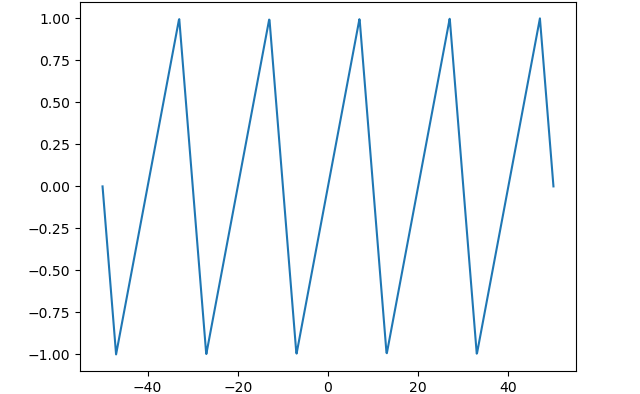
\includegraphics[scale=0.6]{section-02/qc.png}
        \end{center}
\end{enumerate}
